\documentclass[a4paper]{article}
\usepackage[utf8]{inputenc}
\usepackage[T1]{fontenc}
\usepackage[brazil]{babel}
\usepackage{graphicx}

\title{}
\author{}
\date{}

\begin{document}
 \pagestyle{empty}
 \begin{figure}
  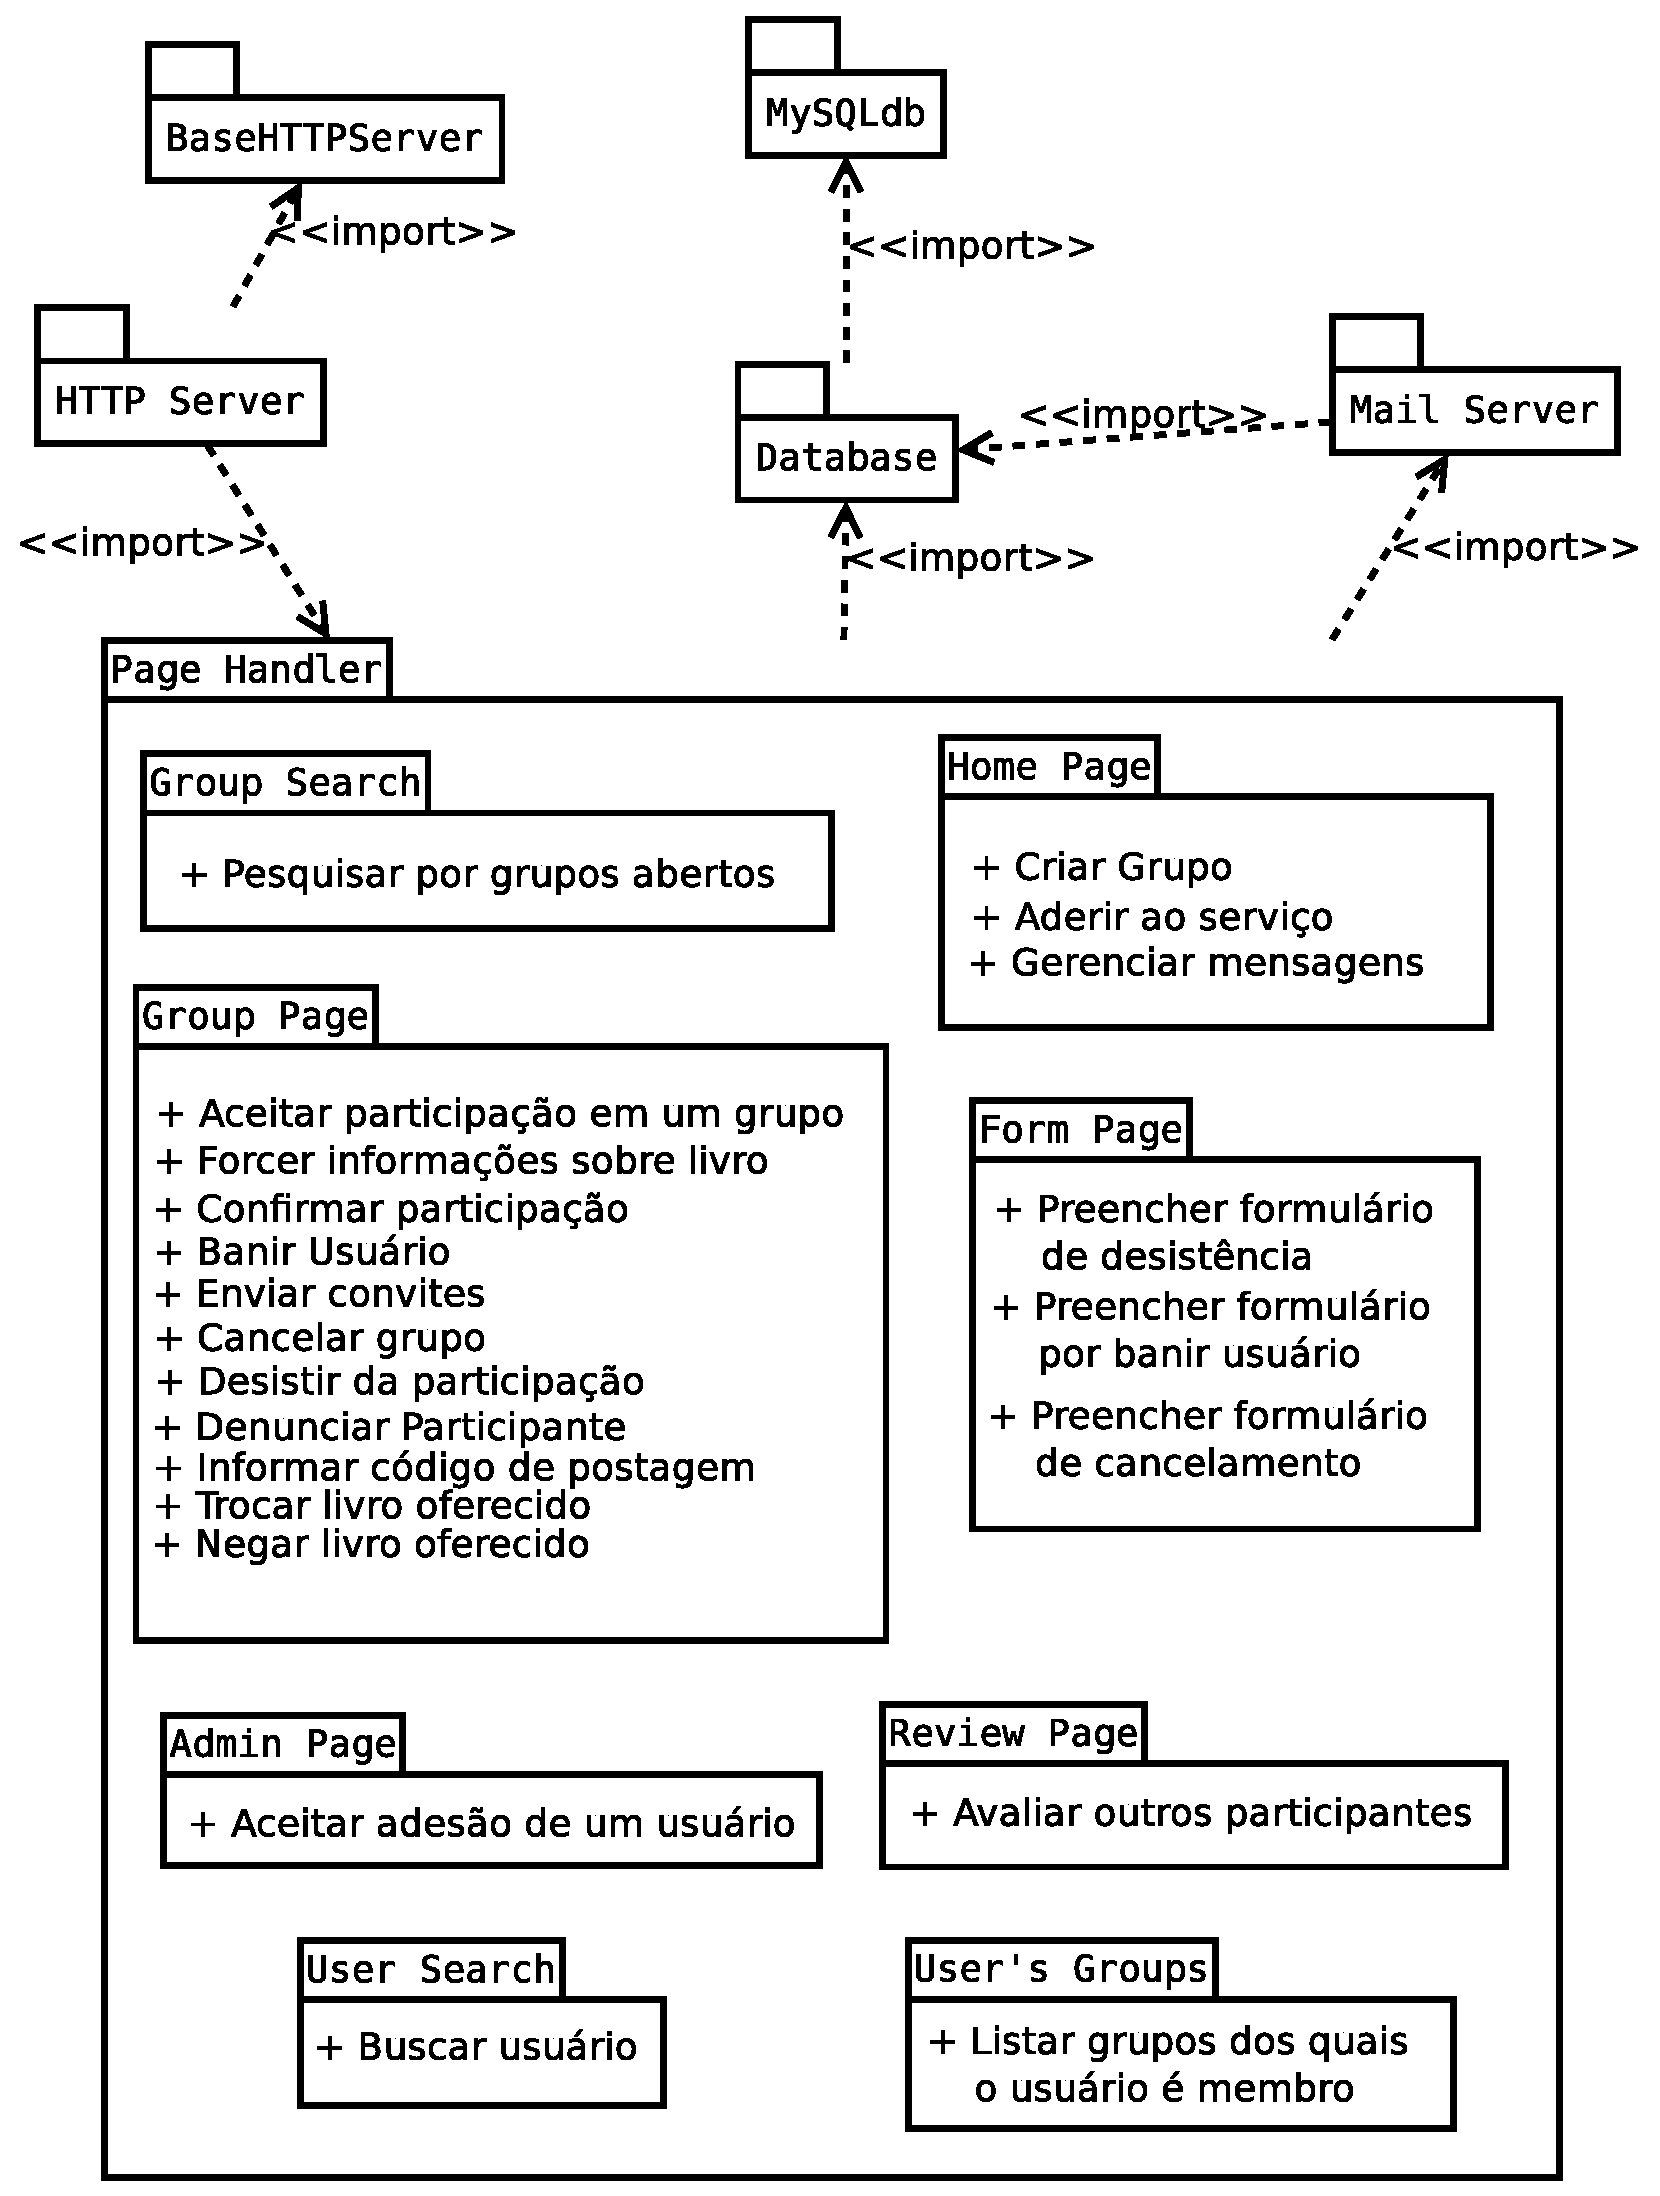
\includegraphics[totalheight=\textheight]{pacotes.eps}
  \caption{Diagrama de Pacotes}
 \end{figure}
 
 \begin{figure}
  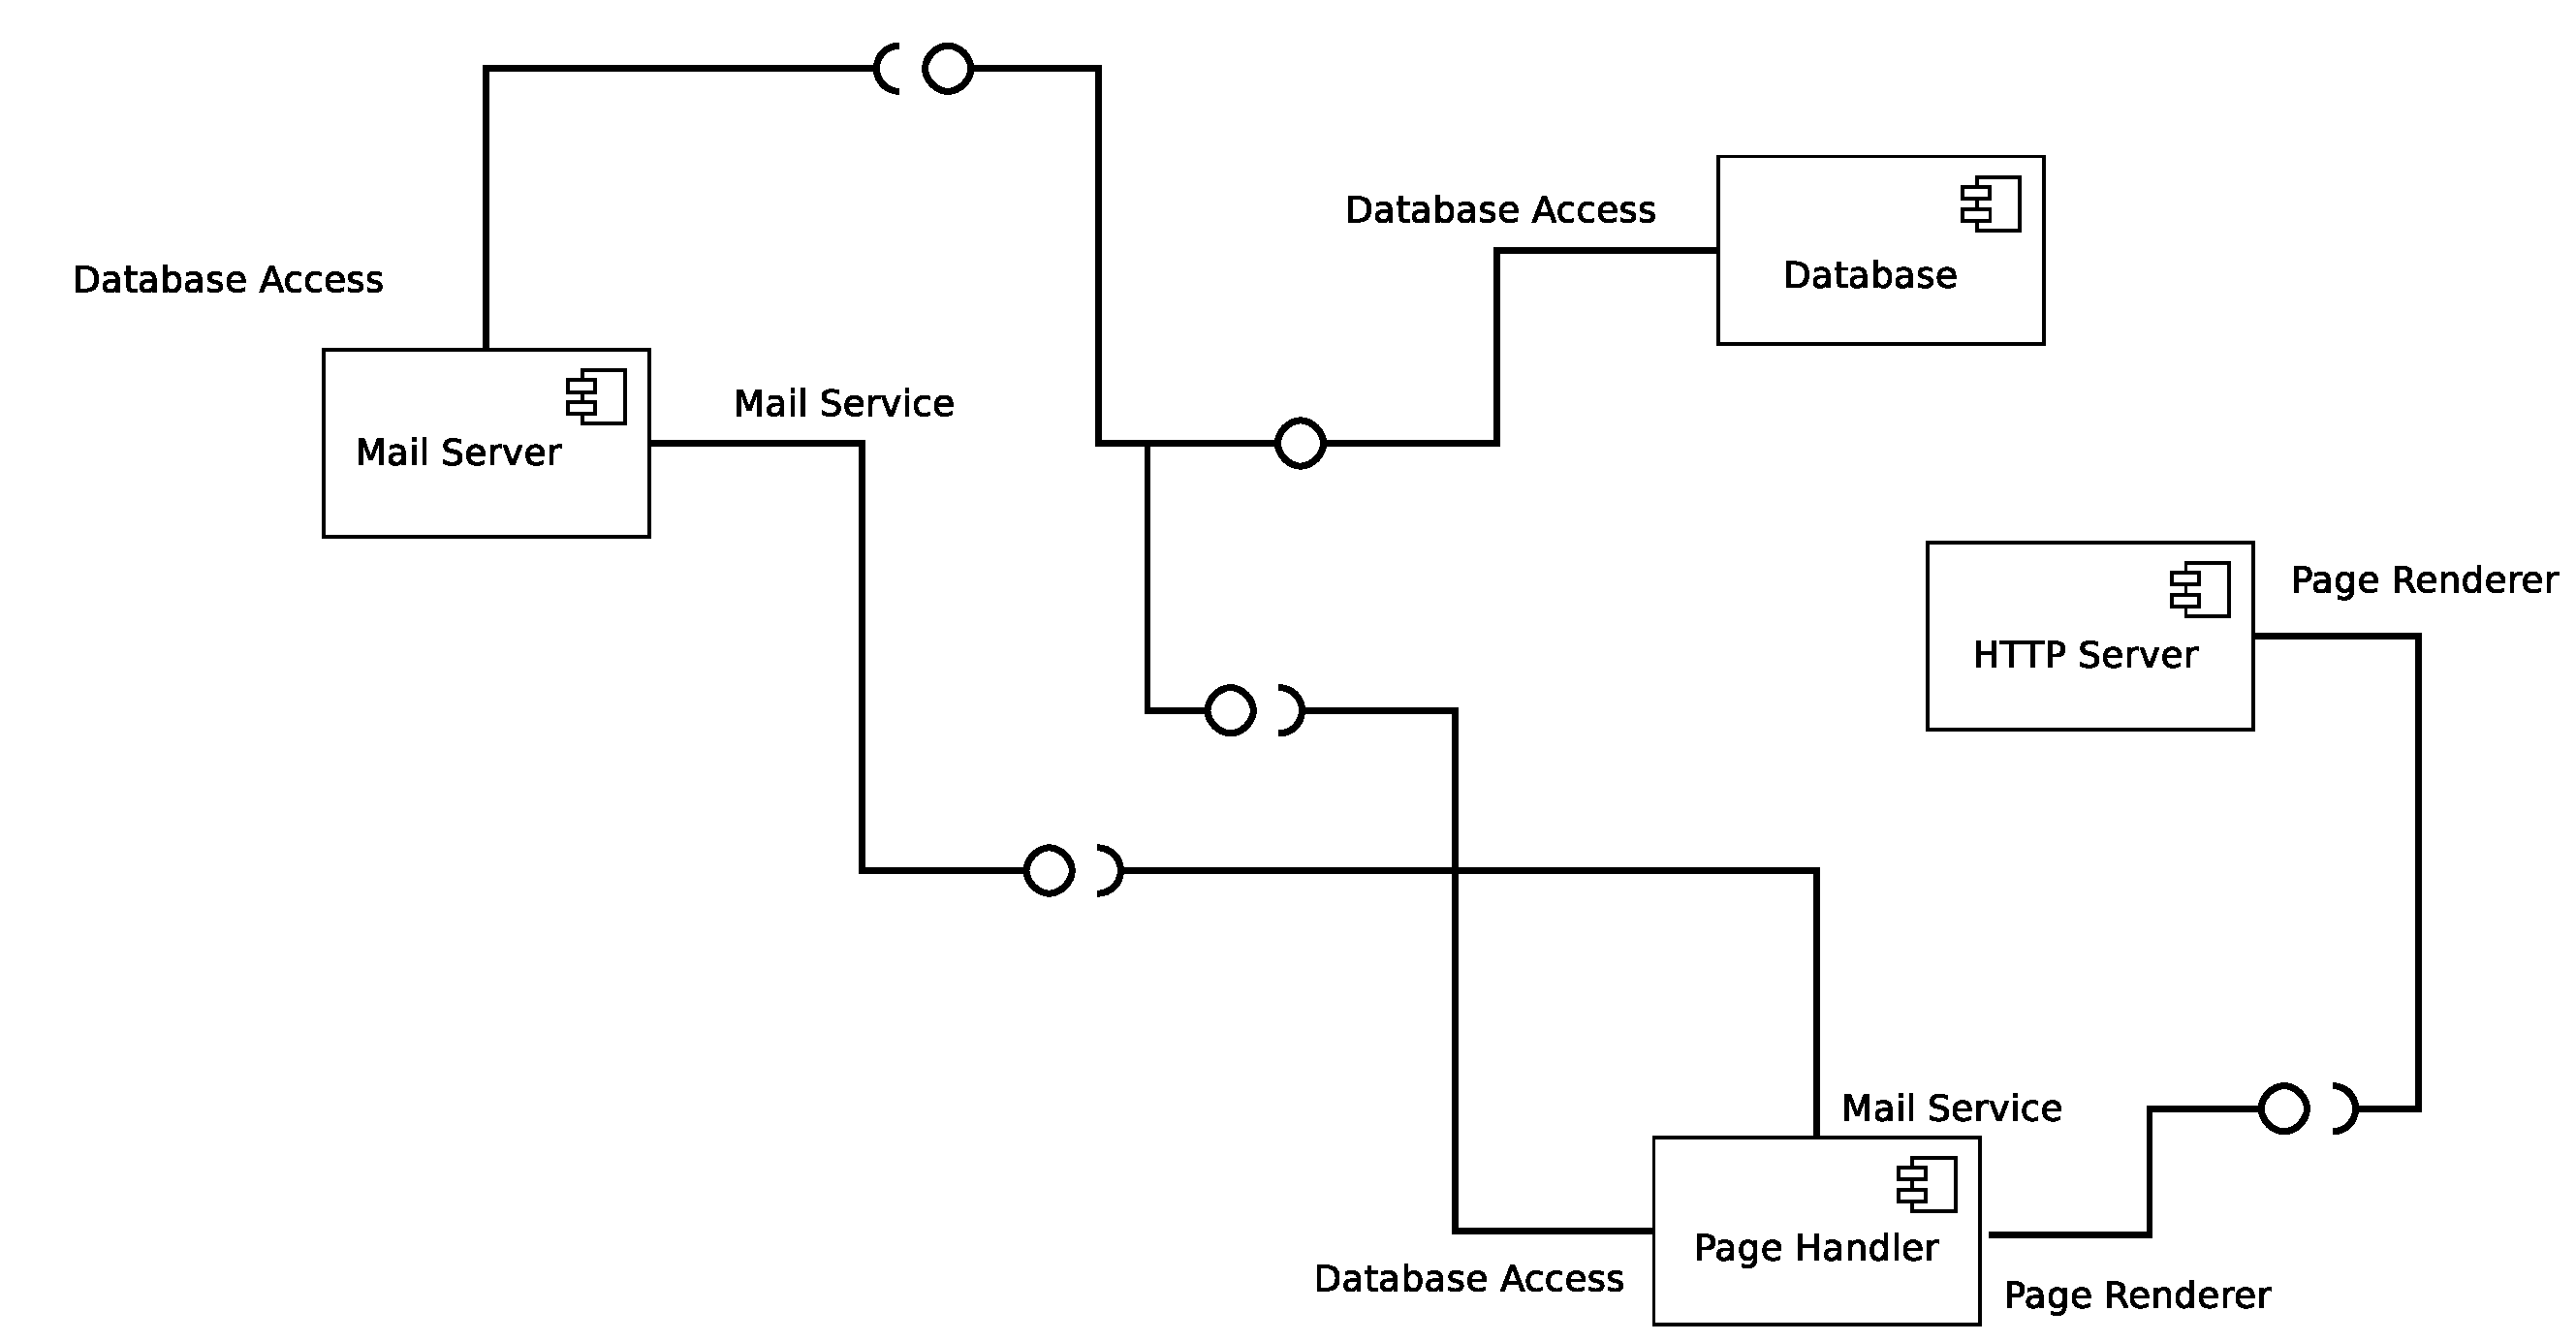
\includegraphics[angle=90,totalheight=\textheight]{componentes.eps}
  \caption{Diagrama de Componentes}
 \end{figure}
 
 \begin{figure}
  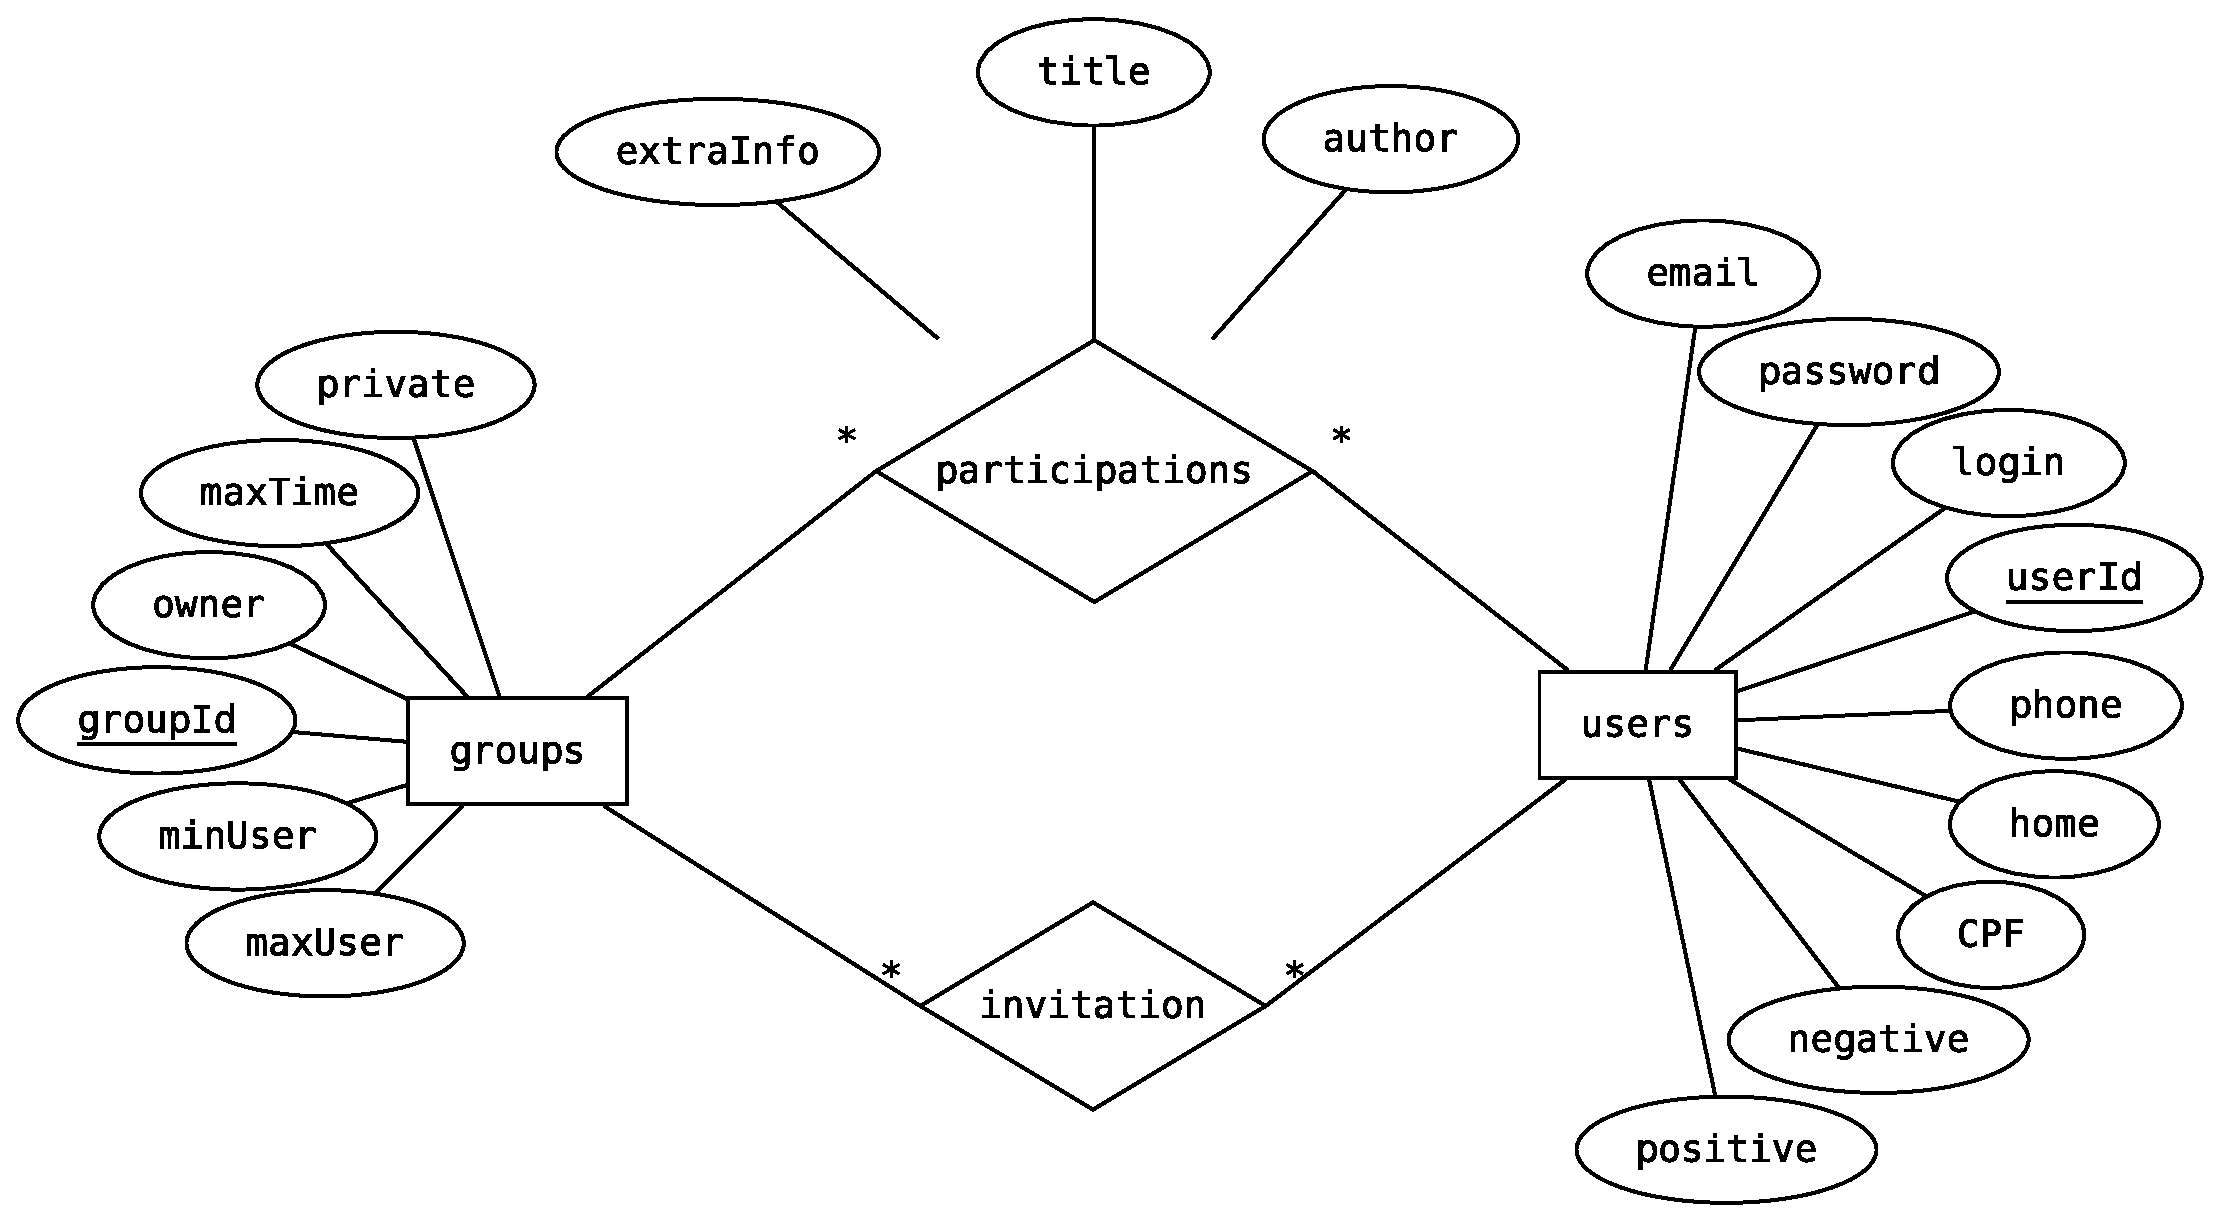
\includegraphics[angle=90,totalheight=\textheight]{modeloER.eps}
  \caption{Modelo Entidade-Relacionamento}
 \end{figure}
 
 \begin{figure}
  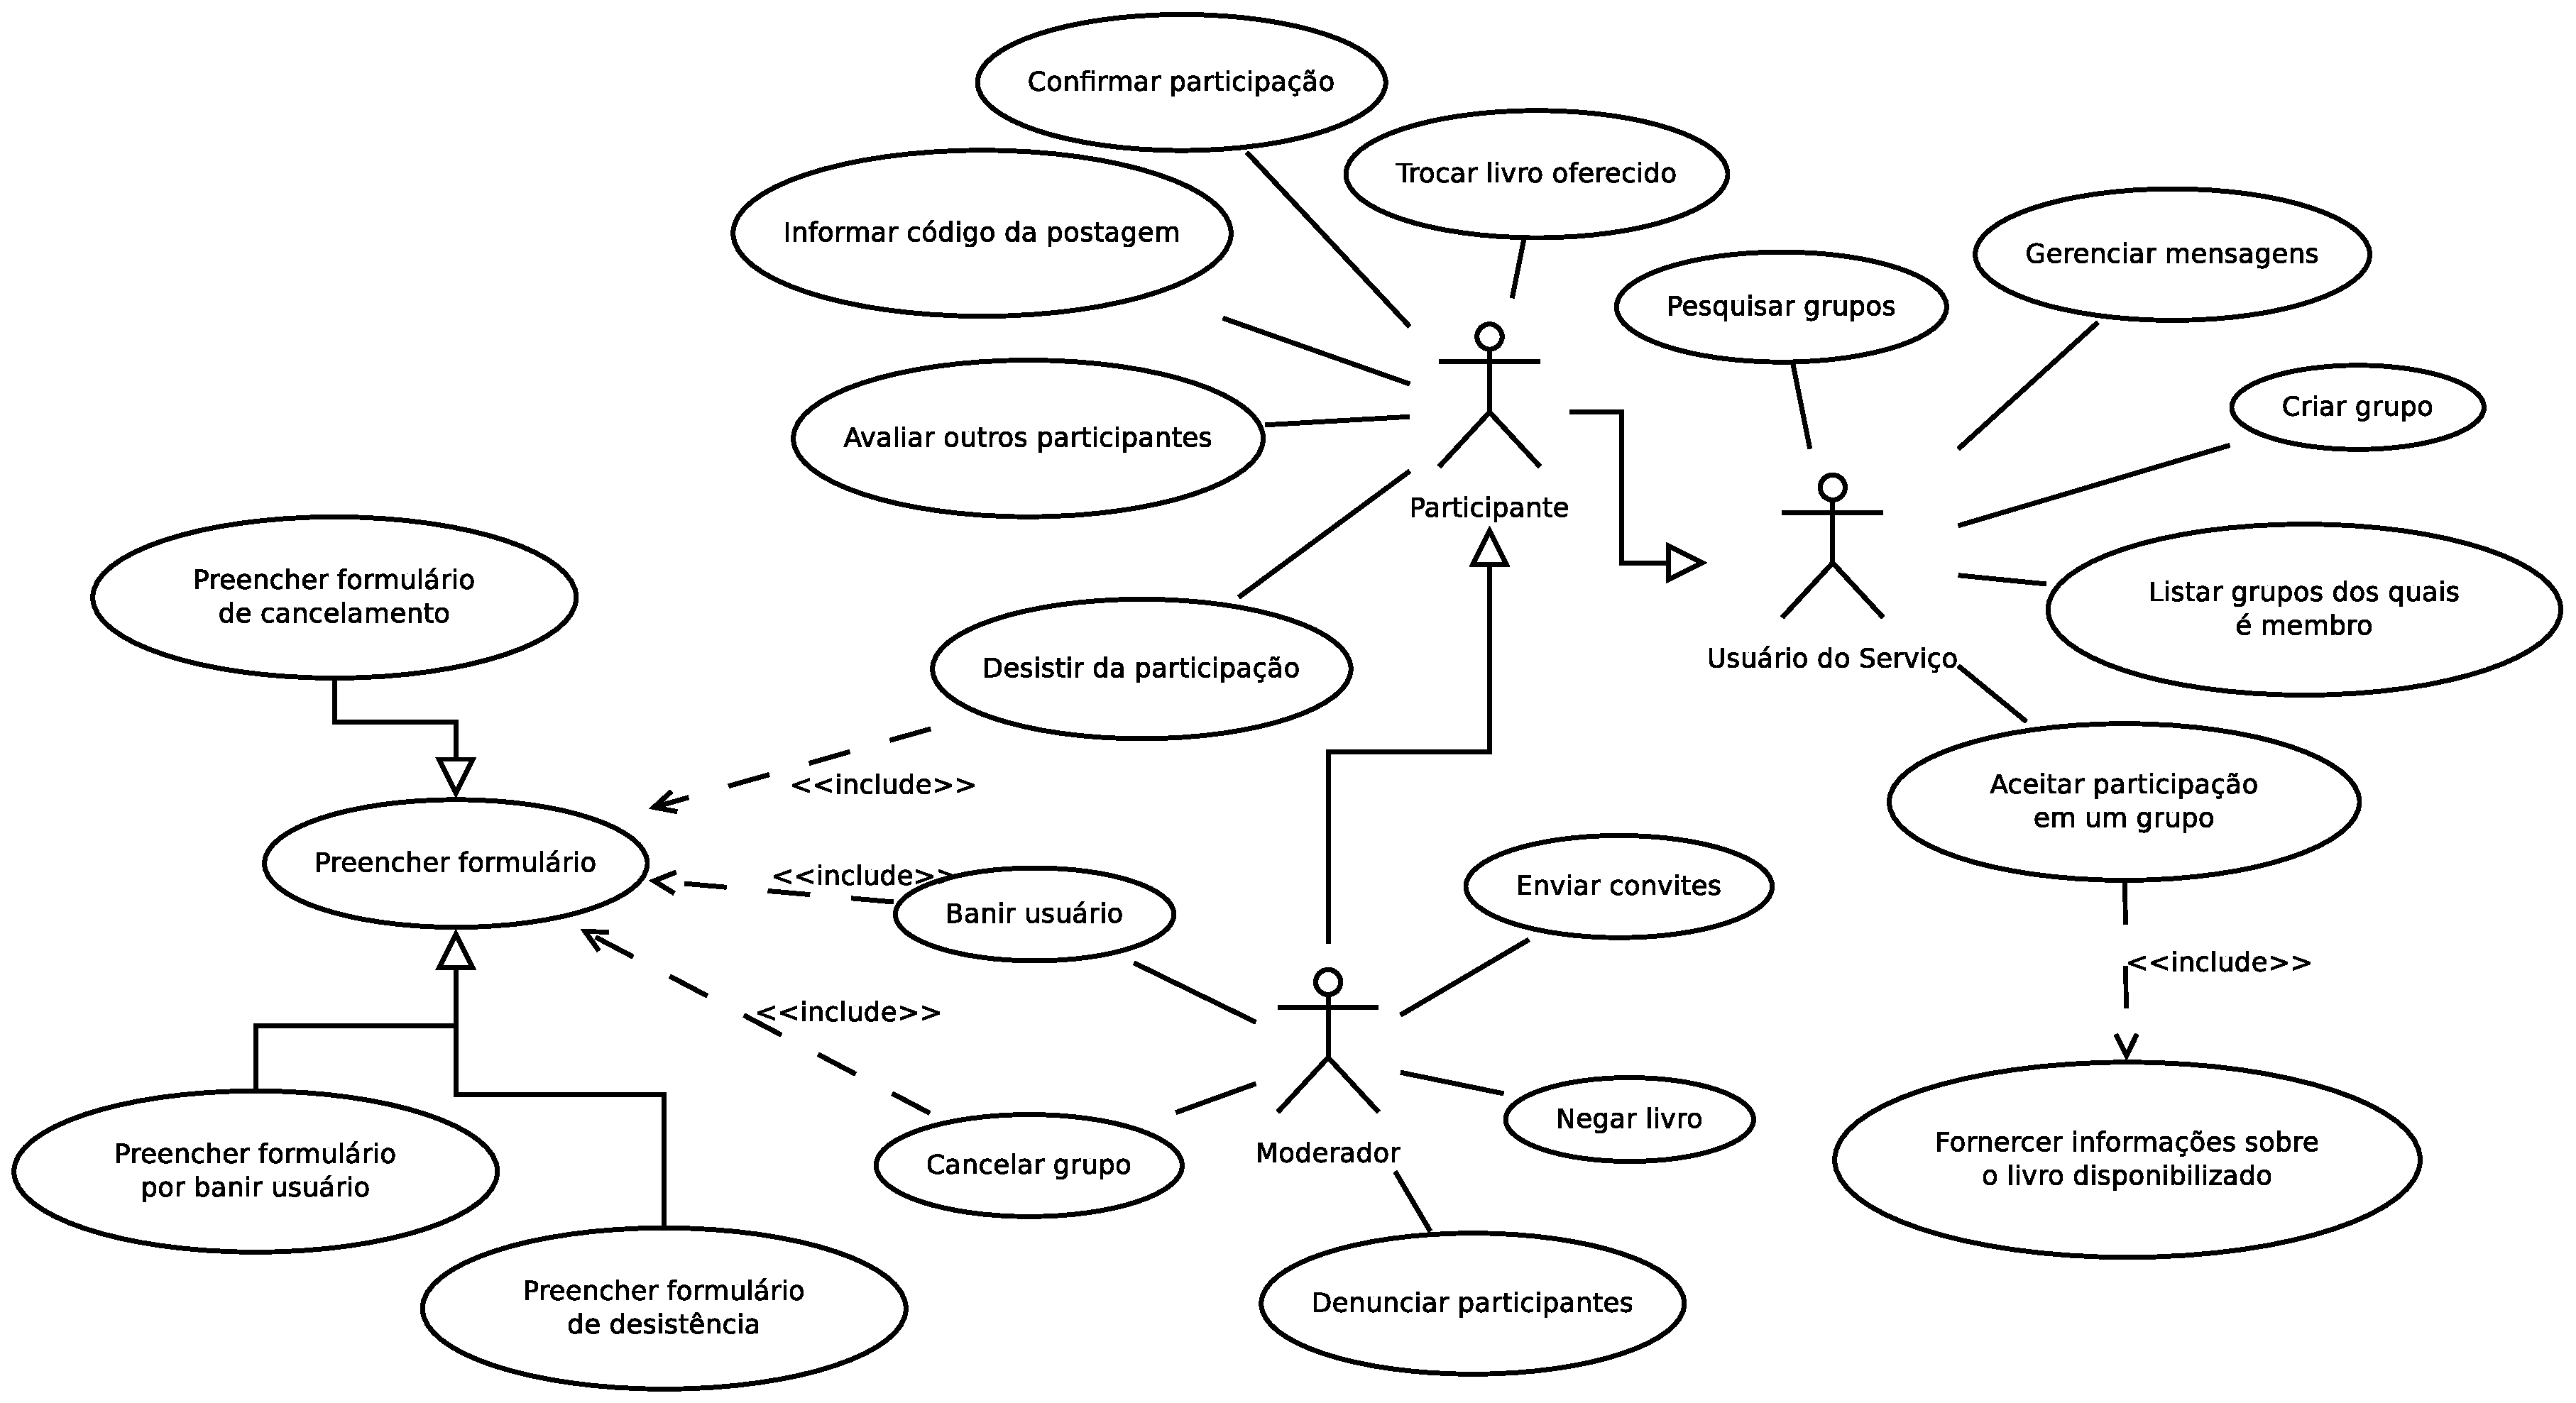
\includegraphics[angle=90,totalheight=\textheight]{casosDeUso.eps}
  \caption{Diagrama de Casos de Uso}
 \end{figure}

 
\end{document}
